\chapter{Turbomeet}
\label{Turbomeet}

Turbomeet ist der Prototyp an dem verschiedene Libraries und Tools getestet werden. Es ist eine Webseite auf der sich Nutzer anmelden können und Meetings mit verschiedenen Zeitslots erstellen können. Für diese Zeitslots kann dann von anderen Nutzern abgestimmt werden. Wenn ein Meeting abgeschlossen wird bzw. die Deadline erreicht wird, werden die Zeitslots mit den meisten Teilnahmen ausgewählt.

\section{Technologien}
\label{Technologies}

Der ausgewählte Technologie Stack ist der T3-Stack:

\begin{itemize}
    \item Next.js
    \item TypeScript
    \item tRPC
    \item TailwindCSS
    \item Prisma
    \item NextAuth.js
\end{itemize}

Neben diesen Technologien werden noch weitere Libraries verwendet, die in den folgenden Abschnitten genauer beschrieben werden.

\subsection{Next.js}

Next.js ist ein serverseitiges JavaScript-Framework, das auf React aufbaut. Es ist dafür ausgelegt, schnelle und skalierbare Anwendungen zu entwickeln. Zu den Funktionen von Next.js gehören:

\begin{itemize}
    \item Serverseitiges Rendern (SSR): Next.js kann die HTML-Ausgabe auf dem Server generieren, was die Ladezeit der Seite verbessert und die Suchmaschinenoptimierung (SEO) erleichtert.
    \item Automatisches Code-Splitting: Next.js teilt automatisch den Code in kleine, optimierte Teile auf, um die Ladezeit der Seite zu reduzieren.
    \item Hot-Module-Replacement: Next.js aktualisiert automatisch den Code, während Sie arbeiten, um einen schnellen Entwicklungsprozess zu ermöglichen.
    \item Static Site Generation (SSG): Next.js kann auch statische Seiten generieren, um schnelle und sichere Websites zu erstellen, die auf einem CDN (Content Delivery Network) gehostet werden können.
\end{itemize}

\subsection{TypeScript}

TypeScript ist eine freie und quelloffene Programmiersprache, die auf JavaScript basiert. Sie ist eine statisch typisierte Sprache, die es Entwicklern ermöglicht, die Typen von Variablen und Funktionen zu definieren. Dadurch können Fehler frühzeitig erkannt und behoben werden. Außerdem können Entwickler mit TypeScript auch die neuesten Funktionen von JavaScript verwenden, ohne auf die Kompatibilität mit älteren Browsern achten zu müssen.

\subsection{tRPC}

tRPC ist ein Open-Source-Framework, das es Entwicklern ermöglicht, API Endpunkte einfach zu definieren und zu erstellen. Mit dem Motto \emph{``Move fast and break nothing. End-to-end typesafe APIs made easy.``} (\citeurl{httpstrpcio_trpctrpc_nodate}) werden die Vorteile von tRPC sehr gut beschrieben. Durch die Nutzung von TypeScript im Backend sowie im Frontend werden Breaking Changes vermieden und die Entwicklung wird beschleunigt. Wenn bestimmte Felder z.B. in der API geändert/entfernt werden, und auf diese im Frontend zugegriffen wird, werden diese direkt mit spezifischen Fehlern annotiert.

Um eine E2E Typensicherheit bei normalen REST und GraphQL APIs zu erhalten muss eine Vielzahl von Tools und Konfiguration vorgenommen werden. Dies ist meist sehr aufwändig und komplex.

\subsection{TailwindCSS}

TailwindCSS ist ein Utility-First CSS-Framework. Das bedeutet, dass es keine vorgefertigten Komponenten wie z.B. Buttons oder Formulare gibt. Stattdessen werden die Komponenten aus einzelnen Utility-Klassen zusammengesetzt. Diese Utility-Klassen sind meist sehr spezifisch und beschreiben nur eine Eigenschaft. So kann z.B. ein Button mit der Klasse \texttt{.bg-blue-500} eine blaue Hintergrundfarbe erhalten. Die Klasse \texttt{.bg-blue-500} beschreibt nur die Hintergrundfarbe und nicht die Größe oder den Abstand zum nächsten Element. Diese Utility-Klassen können dann beliebig kombiniert werden, um die Komponente zu gestalten.

\subsection{Prisma}

Prisma ist ein Open-Source-ORM (Object-Relational Mapping) für Node.js. Es ermöglicht es Entwicklern, Datenbanken zu modellieren und mit der Datenbank zu interagieren. Prisma bietet eine einfache und intuitive API, die es Entwicklern ermöglicht, Datenbankabfragen zu schreiben, ohne sich um die Syntax der Datenbank kümmern zu müssen. Prisma unterstützt eine Vielzahl von Datenbanken, darunter MySQL, PostgreSQL, SQLite und MongoDB.

Prisma generiert automatisch eine TypeScript Typen Definition für die Datenbank. Mithilfe dieser Typen Definition können Entwickler sicherstellen, dass die Datenbank und die API Endpunkte immer synchron sind.

\subsection{NextAuth.js}

NextAuth.js ist ein Open-Source-Framework, das es Entwicklern ermöglicht, Authentifizierung und Autorisierung in Next.js Anwendungen zu implementieren. Es bietet eine einfache und intuitive API, die es Entwicklern ermöglicht, verschiedene Authentifizierungsmethoden zu implementieren, wie z.B. OAuth, E-Mail-Authentifizierung, Passwort-Authentifizierung, Magic-Links, etc.

\subsection{Radix UI}

Wie bereits in dem \hyperref[secsec:radix]{Recherche Kapitel} beschrieben ist Radix UI ein \emph{primitive-first} UI-Framework. Es werden z.B. Komponenten wie Buttons, Inputs und Dialoge bereitgestellt. Diese sind immer bereits mit der Funktionalität und Accessability Features ausgestattet. Außerdem sind die Komponenten un-styled, d.h. sie haben keine vorgefertigte CSS-Klasse. Stattdessen können die Komponenten mit den Utility-Klassen von TailwindCSS gestyled werden.

Alle Komponenten von Radix UI folgen dem \emph{WAI-ARIA} Standard und implementieren die Accessability Patterns der \emph{APG} wie in im Kapitel \ref{secsec:apg_patterns} beschrieben. Dadurch werden den Entwicklern bereits viele Accessability Features zur Verfügung gestellt und es muss nicht jedes Mal alles neu/manuell implementiert werden.

Bestimmte Felder wie z.B. die \texttt{label} eines Inputs können mit einem \texttt{aria-label} versehen werden. Dadurch wird der Input für Screenreader und andere Assistive Technologien lesbar. Diese Werte kann Radix UI nicht automatisch generieren, da es nicht weiß, was in den Feldern steht. Deshalb müssen diese Werte manuell angegeben werden. Aber auch hier hilft Radix UI, indem es in der Dokumenation explizit darauf hinweist, dass diese Werte angegeben werden müssen.

In der Dokumenation zu den einzelnen Komponenten werden außerdem die Accessability Features beschrieben. So wird z.B. bei einem Dialog beschrieben, dass der Dialog mit der Tastatur bedienbar ist und wie dies funktioniert. Außerdem wird beschrieben, dass der Dialog mit einem Screenreader gelesen werden kann. In Abbildung \ref{fig:radix_dialog_keyboard} ist ein Screenshot der Dokumenation zu einem Dialog zu sehen.

\begin{figure}[th]
\centering
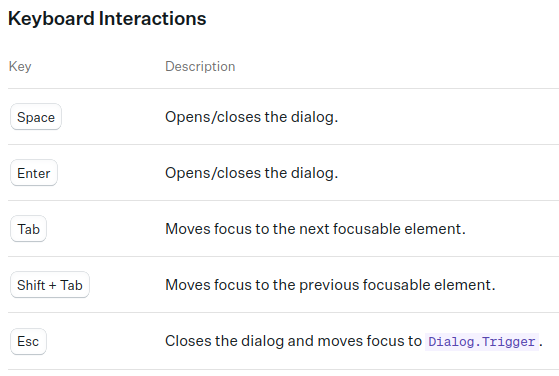
\includegraphics[width=\textwidth]{Figures/radix_dialog_keyboard.png}
\decoRule
\caption[Dialog Accessability Dokumenation]{Radix UI Dialog Accessability Dokumenation}
\label{fig:radix_dialog_keyboard}
\end{figure}

